\begingroup

\let\clearpage\relax
\chapter{Indexability}
\label{chp:apx_indexability}

%\section{Examples and counterexamples}
%
%In this section, we provide a few examples to illustrate the ambiguities in the classical definition of indexability, and to illustrate what can happen for some multichain arms. We also provide the parameters of arms presented in Figure~\ref{fig:illustrate_indexability}.
%
%\subsection{Discussion on the definition of indexability}
%\label{apx:discussion_index}
%
%The classical notion of indexability used in the literature is to say that the optimal policy $\pi^*(\lambda)$ should be non-increasing in $\lambda$. Yet, we argue that this definition has two problems:
%\begin{enumerate}
%    \item What does ``increasing'' mean when $\pi^*(\lambda)$ is not unique? Two possibilities are: for all penalties $\lambda<\lambda'$:
%    \begin{enumerate}
%        \item[($\exists$)] there exist policies $\pi,\pi'$ with $\pi$ optimal for $\lambda$ and $\pi'$ optimal for $\lambda'$ such that $\pi\supseteq\pi'$;
%        \item[($\forall$)] for all policies $\pi,\pi'$ such that  $\pi$ is optimal for $\lambda$ and $\pi'$ is optimal for $\lambda'$, we have $\pi\supseteq\pi'$.
%    \end{enumerate}
%    \item What notion of ``optimality'' should be used? Two possibilities are: 
%    \begin{enumerate}
%       \item[(GO)] ``optimal'' means gain optimal.
%       \item[(BO)] ``optimal'' means Bellman optimal.
%   \end{enumerate}
%\end{enumerate}
%The most problematic choice is the notion of increasingness: Interpretation $(\exists)$ is more permissive: For instance, consider an arm with two states and assume that the optimal policy is $\{1,2\}$ for $\lambda<0$ and is either $\{1\}$ or $\emptyset$ for $\lambda>0$. Interpretation $(\exists)$ says that the arm is indexable while interpretation ($\forall$) says that this arm is not indexable. If the arm is indexable, what should the index of state $1$ be? Any choice $\lambda_1\in[0,+\infty]$ seems reasonable. Saying that the arm is not indexable clarifies the situation. This is why we choose interpretation ($\forall$) in our paper.
%
%In our paper, we choose the combination ($\forall$-BO) because we believe that, for a problem that has transient state, the notion of Bellman optimality is more meaningful than the notion of gain optimality. Also, our combination ($\forall$-BO) allows for more problems to be indexable compared to ($\forall$-GO) and is easier to characterize.
%
%\begin{figure}[ht]
%    \centering
%    \begin{tabular}{ccc}
%        \begin{minipage}{.25\linewidth}
%            \begin{tikzpicture}[on grid, state/.style={circle,draw}, >= stealth', auto, prob/.style = {inner sep=1pt,font=\scriptsize}]
%                \node[state,color=blue]  (A) {$2$};
%                \node[state,color=blue]  (B) [left =1.5cm of A]   {$1$};
%                \path[->]
%                    (A) edge[loop above,color=black]  node{$1{-}\lambda$} (A)
%                    (A) edge[loop right, color=red, dashed]     node{$1$} (A)
%                    (B) edge[bend left, color=black]     node{$1{-}\lambda$} (A)
%                    (B) edge[bend right, color=red, dashed]     node[below]{$1$} (A);
%            \end{tikzpicture}
%        \end{minipage}
%        &
%        \begin{minipage}{.25\linewidth}
%            \begin{tikzpicture}[on grid, state/.style={circle,draw}, >= stealth', auto, prob/.style = {inner sep=1pt,font=\scriptsize}]
%            \node[state,color=blue]  (A) {$2$};
%            \node[state,color=blue]  (B) [left =1.5cm of A]   {$1$};
%            \path[->]
%                (A) edge[loop above,color=black]  node{$1{-}\lambda$} (A)
%                (A) edge[loop right, color=red, dashed]     node{$1$} (A)
%                (B) edge[color=black]     node{$1{-}\lambda$} (A)
%	            (B) edge[loop left, color=red, dashed]     node[left]{$1$} (B);
%            \end{tikzpicture}
%        \end{minipage}\\
%        (a) & (b)
%    \end{tabular}
%    
%    \caption{Ambiguous examples: All transitions are deterministic and labels on transitions indicate rewards. Solid black arrows correspond to the action ``activate'' and dashed red arrows to the action ``rest''.
%}
%    \label{fig:ambiguous_example}
%\end{figure}
%
%We illustrate these different definitions in Figure~\ref{fig:ambiguous_example}. For example (a):
%\begin{itemize}
%    \item The gain optimal policies are $\{1,2\}$ and $\{2\}$ for $\lambda<0$, and $\{1\}$ and $\emptyset$ for $\lambda>0$: According to the interpretation~$(\exists)$, the problem should be indexable but the index for state $1$ is unclear. According to the interpretation~$(\forall)$, the problem should not be indexable.
%    \item The Bellman optimal policy is $\{1,2\}$ for $\lambda<0$, and $\emptyset$ for $\lambda>0$. According to our definition, ($\forall$-BO), the problem is indexable and the indices are $\lambda_1=\lambda_2=0$.
%\end{itemize}
%For example (b), the Bellman optimal and gain optimal policies are identical and equal to the gain optimal policies of example (a). Hence, example (b) is not indexable according to our definition. The output of our algorithm for this problem is "multi-chain". 
%%However, the intuition would suggest that the index for this problem should be $\lambda_1=\lambda_2=0$. This is what would have happened if we had used the notion of \emph{bias optimal} policy that is stronger than the notion of Bellman optimal policy. Yet, this would not solve the ambiguity of example (c) for which the index of state $1$ is not clear unless one would use an even  stronger notion of optimality (such as the notion of \emph{Blackwell optimality} discussed in \cite[Chapter~10]{putermanMarkovDecisionProcesses1994}). In this paper, we keep the notion of Bellman optimal and we do not use these stronger definition because computing a Blackwell-optimal policy is, to the best of our knowledge, not computable in $O(n^3)$ (the complexity of computing Blackwell-optimal policies is unknown to this date). Hence, in this paper we use the notion of Bellman optimality that we think is the best tradeoff between expressiveness and calculability.
%
%Note that if the distinction between (BO) and (GO) disappears for discounted problems, the distinction between ($\forall$) and ($\exists$) remains.
%
%\subsection{Multichain arms and infinite indices}
%\label{apx:multichain}
%
%\begin{figure}[ht]
%    \centering
%    \begin{minipage}{.35\linewidth}
%        \centering
%        \begin{tikzpicture}[on grid, state/.style={circle,draw}, >= stealth', auto, prob/.style = {inner sep=1pt,font=\scriptsize}]
%            \node[state,color=blue]  (A) {$2$};
%            \node[state,color=blue]  (B) [left =1.5cm of A]   {$1$};
%            \path[->]
%            (A) edge[loop right,color=black]  node{$1-\lambda$} (A)
%            (A) edge[loop above, color=red, dashed]     node{$1$} (A)
%            (B) edge[color=black]     node{$1-\lambda$} (A)
%            (B) edge[loop above, color=red, dashed]     node{$0$} (B);
%        \end{tikzpicture}\\
%        (a) Our algorithm returns ``indexable''.
%    \end{minipage}\qquad 
%    \begin{minipage}{.35\linewidth}
%        \centering
%        \begin{tikzpicture}[on grid, state/.style={circle,draw}, >= stealth', auto, prob/.style = {inner sep=1pt,font=\scriptsize}]
%            \node[state,color=blue]  (A) {$2$};
%            \node[state,color=blue]  (B) [left =1.5cm of A]   {$1$};
%            \path[->]
%            (A) edge[loop right,color=red, dashed]  node{$0$} (A)
%            (A) edge[loop above, color=black]     node{$1-\lambda$} (A)
%            (B) edge[color=red, dashed]     node{$0$} (A)
%            (B) edge[loop above, color=black]     node{$-\lambda$} (B);
%        \end{tikzpicture}\\
%        (b) Our algorithm returns ``multichain''.
%    \end{minipage}
%    
%    \caption{Example of an indexable multichain problem with infinite Whittle index. Transitions are deterministic and labels on edges indicate rewards (for the $\lambda$-penalized arm). Solid black transitions correspond to action ``activate''  and dashed red to the action ``rest''.}
%    \label{fig:example_multichain}
%\end{figure} 
%
%Consider the two examples of Figure~\ref{fig:example_multichain}. The examples are multichain because policy $\emptyset$ has two irreducible classes for example (a) and policy $\{1,2\}$ has two irreducible classes for example (b). These two problems are indexable:
%\begin{itemize}
%    \item For (a), the Bellman optimal policy for $\lambda<0$ is $\{1,2\}$ and $\{1\}$ for $\lambda>0$. The indices are $\lambda_2=0$ and $\lambda_1=+\infty$.
%    \item For (b), the  Bellman optimal policy is $\{2\}$ for $\lambda<0$  and $\{1,2\}$ for $\lambda>0$. The indices are $\lambda_1=0$ and $\lambda_2=-\infty$.
%\end{itemize}
%For the first example, our algorithm returns the correct indices because the constructed policies are $\pi^1:=\{1,2\}\supsetneq\pi_2:=\{1\}$ and they are both unichain.  For the second example, our algorithm will start with the policy $\{1,2\}$ and will stop by saying that this example is multichain.

\subsection{Parameters for the example of Figure~\ref{fig:illustrate_indexability}}
\label{apx:non_indexable_example}

The numerical data of the indexable arm presented in Figure~\ref{fig:illustrate_vf} is
\begin{equation*}
    \mP^0{=}\begin{bmatrix}
        0.363 & 0.503 & 0.134 \\
        0.082 & 0.754 & 0.164 \\
        0.246 & 0.029 & 0.724
    \end{bmatrix}
    \mP^1{=}\begin{bmatrix}
        0.172 & 0.175 & 0.653 \\
        0.055 & 0.931 & 0.014 \\
        0.155 & 0.627 & 0.218
    \end{bmatrix}
    \vr^1{=}\begin{bmatrix}
        0.441 \\
        0.803 \\
        0.426
    \end{bmatrix}
    \vr^0{=}\vzero
\end{equation*}

\noindent
The numerical data of the non-indexable arm presented in Figure~\ref{fig:illustrate_non_indexable} is

\begin{equation*}
    \mP^0{=}\begin{bmatrix}
        0.005 & 0.793 & 0.202 \\
        0.027 & 0.558 & 0.415 \\
        0.736 & 0.249 & 0.015
    \end{bmatrix}
    \mP^1{=}\begin{bmatrix}
        0.718 & 0.254 & 0.028 \\
        0.347 & 0.097 & 0.556 \\
        0.015 & 0.956 & 0.029
    \end{bmatrix}
    \vr^1{=}\begin{bmatrix}
        0.699 \\
        0.362 \\
        0.715
    \end{bmatrix} \vr^0{=}\vzero
\end{equation*}

%\section{Technical lemmas}
%
%\subsection{Unicity of Bellman optimal policy}
%\label{apx:unicity_BO}
%
%\subsubsection{Definition and notation}
%
%We are given a MDP $\langle\gS,\gA,r,P\rangle$ with finite state and action spaces.
%As shown in \cite[Chapter~9]{puterman2014markov}, for such a MDP, the optimal gain $\vg^*$ is a vector that satisfies the \emph{multichain optimality equations}: for each $i\in\gS$:
%\begin{align}
%    \max_{a\in\gA}{\Big(\sum_{j\in\gS}P^a_{ij}g^*_j-g^*_i\Big)} =0 \label{eq:gain_max}\\
%    \max_{a\in\gA}{\Big(r^a_i -g^*_i +\sum_{j\in\gS}P^a_{ij}h_j-h_i\Big)} =0. \label{eq:bias_max}
%\end{align}
%%where $\gA_i\subseteq\gA$ is the set of actions that are available at state $i$, and $\vh$ is a bias vector.
%This system uniquely determines the optimal gain that we denote by $\vg^*$.
%However, vector $\vh$ is not uniquely determined by the system.
%In the following, we denote by $H$ the set of bias vector $\vh$ such that $(\vg^*,\vh)$ is a solution of the optimality equations \eqref{eq:gain_max}--\eqref{eq:bias_max}. A policy $\pi$ is Bellman optimal if there exists a bias $\vh\in H$ such that policy $\pi$ attains the maximum \eqref{eq:bias_max}, \emph{i.e.}, for all $i\in\gS$:
%\begin{align*}
%    \pi_i \in \argmax_{a\in\gA}{\Big(r^a_i -g_i +\sum_{j\in\gS}P^a_{ij}h_j-h_i\Big)} = \argmax_{a\in\gA}{\Big(r^a_i +\sum_{j\in\gS}P^a_{ij}h_j\Big)}.
%\end{align*}
%
%For a given policy $\pi:\gS\mapsto\gA$, we denote by $\vr^\pi$ and $\mP^\pi$ the reward vector and state transition matrix under policy $\pi$: $r^\pi_i=r^{\pi_i}_{i}$ and $P^\pi_{ij} = P^{\pi_i}_{ij}$. Let $\vg^\pi,\vh^\pi\in\real^{\vert \gS\vert}$ be a solution of the following system:
%\begin{align}
%    \vg^\pi - \mP^{\pi}\vg^\pi &=\vzero \label{eq:gain_eval}\\
%    \vr^{\pi}  - \vg^\pi+\mP^{\pi}\vh^\pi  -\vh^\pi &= \vzero \label{eq:bias_eval1}.
%\end{align}
%The vector $\vg^\pi$ is uniquely determined by this system of equations and is called the long-term average reward or gain of policy $\pi$. The vector $\vh^\pi$ is unique up to an element of the null space of $(\mI-\mP^\pi)$. Such a vector $\vh^\pi$ is called a bias of policy $\pi$.
%
%If $(\vg^\pi, \vh^\pi)$ is a solution of \eqref{eq:gain_eval} and \eqref{eq:bias_eval1}, then the advantage of action $a$ over the action $\pi_i$ when the MDP is in state $i$ is given by:
%\begin{align*}
%    B^a_i(\vh^\pi) &:=r^a_i +\sum_{j\in\gS}P^a_{ij}h^\pi_j -g^{\pi}_i -h^\pi_i\\
%    &= r^a_i - r^{\pi_i}_i +\sum_{j\in\gS}(P^a_{ij}-P^{\pi_i}_{ij})h^\pi_j
%\end{align*}
%%This advantage function is well-defined when the policy $\pi$ is unichain. 
%% Hence, for $\vg^*$ and any $\vh\in H$, $B^a_i(\vh) =r^a_i -g^*_i +\sum_{j\in\gS}P^a_{ij}h_j-h_i$ is the advantage of action $a$ over the best action when the MDP is in state $i$. This quantity is always negative and null if the action $a$ is optimal, $B^a_i(\vh)\le0$ for all $\vh\in H$.
%
%We recall the two notions of optimality:
%\begin{itemize}
%    \item A policy $\pi$ is gain optimal if its gain $\vg^\pi$ equals $\vg^*$.
%    \item A policy $\pi$ is Bellman optimal if $\vg^*=\mP^\pi \vg^*$ and if there exists a bias $\vh^\pi$ that is a solution of \eqref{eq:bias_eval1} and also \eqref{eq:bias_max}.
%\end{itemize}
%Recall that a Bellman optimal policy is also gain optimal.
%
%Note that by the definition the advantage $B(\cdot)$, a policy is Bellman optimal if $\vg^*=\mP^\pi \vg^*$ and if there exists $\vh\in H$ such that $B^{\pi_i}_i(\vh)=0$.
%
%\paragraph*{Useful notations}
%
%Let $\pi:\gS\to\gA$ be a policy. We say that a state is recurrent for $\pi$ if it is recurrent for the Markov chain whose transition matrix is $\mP^\pi$. In other words, a state $i\in\gS$ is recurrent if when the chain starts in $i$ at time $0$, it almost surely visits the state $i$ at some time $t\ge1$.  We denote by $\gR^\pi$ the set of recurrent states of policy $\pi$. 
%
%We also define $\bar{\mP}^\pi$ as the Cesaro limit of the sequence $\{(\mP^\pi)^t\}_{t=1}$:
%\begin{align*}
%    \bar{\mP}^\pi:=\lim_{T\to\infty}\frac1T\sum_{t=1}^T(\mP^\pi)^{t-1}.
%\end{align*}
%From \cite[Section~A.4 of Appendix~A]{puterman2014markov}, the matrix  $\bar{\mP}^\pi$ exists and has the following properties:
%\begin{itemize}
%    \item $\bar{\mP}^\pi$ is a stochastic matrix, and satisfies $\mP^\pi \bar{\mP}^\pi = \bar{\mP}^\pi\mP^\pi =\bar{\mP}^\pi$.
%    \item For all state $i,j$, if $j\not\in\gR^\pi$, then $\bar{P}^\pi_{ij}=0$.
%    \item If $\pi$ is unichain, then the rows of $\bar{\mP}^\pi$ are identical. 
%\end{itemize}
%
%\subsubsection{Characterization of gain optimal policies}
%
%The following lemma characterizes gain optimal policy by showing that the policy must satisfies \eqref{eq:bias_max} on their recurrent states.
%\begin{lem}
%    \label{lem:opt_pol}
%    Let $\pi:\gS\mapsto\gA$ be a policy and recall that $\gR^\pi$ is the set of recurrent states of policy $\pi$.
%    The three properties below are equivalent.
%    \begin{enumerate}[label=(\roman*)]
%        \item \label{it:opt_pol1} $\mP^\pi\vg^*=\vg^*$ and for all $\vh\in H$, $B^{\pi_i}_i(\vh)=0$ for all $i\in\gR^\pi$
%        \item \label{it:opt_pol2} $\mP^\pi\vg^*=\vg^*$ and for some $\vh\in H$, $B^{\pi_i}_i(\vh)=0$ for all $i\in\gR^\pi$
%        \item \label{it:opt_pol3} $\pi$ is gain optimal.
%    \end{enumerate}
%\end{lem}
%\begin{proof}
%    \ref{it:opt_pol1} $\Rightarrow$ \ref{it:opt_pol2} is trivial.
%
%    \ref{it:opt_pol2} $\Rightarrow$ \ref{it:opt_pol3}: By definition of $B_i^a(\vh)$, we have $r^{\pi}_i-g^*_i = h_i-\sum_{j\in\gS} P^{\pi}_{ij}h_j$ for any recurrent state $i$ of $\pi$.  Multiply this with $\bar{P}^\pi_{ki}$ and sum over $i\in\gS$ (if $i$ is not recurrent, then $\bar{P}^\pi_{ki}=0$) gives
%    \begin{align*}
%        \sum_{i\in\gS} \bar{P}^\pi_{ki}(r^{\pi}_i-g^*_i) = \sum_{i\in\gS} \bar{P}^\pi_{ki}h_i - \underbrace{\sum_{i\in\gS} \bar{P}^\pi_{ki}\sum_{j\in\gS} P^{\pi}_{ij}h_j}_{=\sum_{j\in\gS} \bar{P}^\pi_{kj}h_j \text{ since $\bar{\mP}^\pi\mP^\pi=\bar{\mP}^\pi$.}}
%        &= \vzero.
%    \end{align*}
%    By Theorem~8.2.6 of \cite{puterman2014markov}, the average reward of $\pi$ is $\bar{\mP}^\pi r^\pi$. The above equation shows that $\bar{\mP}^\pi\vr^\pi = \bar{\mP}^\pi\vg^*$. Moreover, the assumption  $\mP^\pi\vg^*=\vg^*$ implies that $\bar{\mP}^\pi\vg^*=\vg^*$ which in turn implies that $\bar{\mP}^\pi\vr^\pi=\vg^*$. This shows that the average reward of $\pi$ is $\vg^*$ and therefore $\pi$ is gain optimal.
%    % So, we have $\mP^\pi\vg^*=\vg^*$ and $\bar{\mP}^\pi(\vr^\pi-\vg^*)=\vzero$.
%
%    \ref{it:opt_pol3} $\Rightarrow$ \ref{it:opt_pol1}: If $\pi$ is gain optimal, then $\mP^\pi \vg^*=\vg^*$ and $\bar{\mP}^\pi(\vr^\pi-\vg^*)=\vzero$. The latter rewrites as $\sum_{i\in\gS}\bar{P}^\pi_{ki}(r^{\pi}_i-g^*_i) =0$ for all state $k$. Let $\vh\in H$ be an optimal bias.  For all state $k$, we have    
%    \begin{align}
%        \label{eq:apx_proof_H}
%        \sum_{i\in\gS}\bar{P}^\pi_{ki}B^{\pi_i}_i(\vh) = \sum_{i\in\gS}\bar{P}^\pi_{ki}(r^{\pi}_i-g^*_i +\sum_{j\in\gS}P^{\pi}_{ij}h_j -h_i) &=0.
%    \end{align}
%    As $\vh$ satisfied \eqref{eq:bias_max}, for all action $a$, we have $B^{a}_i(\vh) \le0$ for all states $i\in\gS$ and in particular $B^{\pi_i}_i(\vh) \le0$. This shows that for any state $i$ such that $\bar{P}^\pi_{ki}>0$, one must have $B^{\pi_i}_i(\vh) =0$. Such state $i$ are the recurrent states of $\pi$. This shows that $B^{\pi_i}_i(\vh) =0$ for all $i\in\gR^\pi$.
%\end{proof}
%
%\subsubsection{Characterization of Bellman optimal policies}
%
%The previous lemma shows that a policy is gain optimal if and only if the actions for the recurrent states of the policy satisfy \eqref{eq:bias_max}.
%The following lemma shows the relationship between two policies that are unichain and satisfy \eqref{eq:bias_max} on all states.
%
%\begin{lem}
%    \label{lem:equi_bias}
%    Suppose that two policies $\pi$ and $\theta$ are Bellman optimal, unichain and have at least one common recurrent state: $\gR^\pi\cap\gR^\theta\neq\emptyset$.
%    
%    Then for any $\vh^\pi$ and $\vh^\theta$ solutions of \eqref{eq:bias_eval1} for $\pi$ and $\theta$ respectively, there exists a constant $c$ such that for all state $i$: $h^\pi_i -h^\theta_i =c$. Moreover, in this case, ${B_i^{\theta_i}(\vh^\pi)=B_i^{\pi_i}(\vh^\theta)=0}$ for all $i$.
%\end{lem}
%\begin{proof}
%    Since $\pi$ and $\theta$ are Bellman optimal, $\vh^\pi,\vh^\theta\in H$.
%    In consequence, we have
%    \begin{align*}
%        \vh^\pi \ge \vr^\theta -\vg^* +\mP^\theta\vh^\pi.
%    \end{align*}
%    By Lemma~\ref{lem:opt_pol}~\ref{it:opt_pol1}, the above inequality is an equality for all $i\in\gR^\theta$ because $\theta$ is gain optimal.
%
%    As $\vh^\theta$ satisfies \eqref{eq:bias_eval1}, we have
%    \begin{align*}
%        \vh^\theta -\vh^\pi &\le \vr^\theta -\vg^* +\mP^\theta\vh^\theta -(\vr^\theta -\vg^* +\mP^\theta\vh^\pi) = \mP^\theta(\vh^\theta -\vh^\pi),
%    \end{align*}
%    with equality for all state $i\in\gR^\theta$. This shows that for all $t$, $\vh^\theta -\vh^\pi\le (\mP^\theta)^t(\vh^\theta -\vh^\pi)$ which implies that $\vh^\theta -\vh^\pi\le \bar{\mP}^\theta(\vh^\theta -\vh^\pi)$ with equality for all states $i\in\gR^\theta$. Similarly, $\vh^\pi -\vh^\theta \le \bar{\mP}^\pi(\vh^\pi -\vh^\theta)$ with equality for any state $i\in\gR^\pi$.
%
%    Let $c^\pi_i=\sum_{j\in\gS}\bar{P}^\pi_{ij}(h_j^\pi-h_j^\theta)$ and $c^\theta_i=\sum_{j\in\gS}\bar{P}^\theta_{ij}(h_j^\pi-h_j^\theta)$. By what we have just shown, for all state $i$, we have
%    \begin{align*}
%        c^\theta_i \underbrace{\le}_{\text{equality if $i\in\gR^\theta$}} h_i^\pi-h_i^\theta \underbrace{\le}_{\text{equality if $i\in\gR^\pi$}} c^\pi
%    \end{align*}
%    As both policies are unichain, $c^\pi_i$ and $c^\theta_i$ do not depend on $i$.  Moreover, if there exists $i\in\gR^\theta\cap\gR^\pi$, we have $c^\pi_i=c^\theta_i =: c$. In consequence,  $h_i^\pi-h_i^\theta=c$ for all state $i$. 
%\end{proof}
%
%
%\subsubsection{Unicity of Bellman optimal policy}
%\label{ssec:unicity}
%
%\begin{lem}
%    \label{lem:unicity_BO}
%    Let $\pi$ be a Bellman optimal policy that is unichain. If $\pi$ is not the unique Bellman optimal policy, then there exists a state $i$ and an action $a\neq\pi_i$ such that $B_i^a(\vh^\pi)=0$.
%\end{lem}
%\begin{proof}
%    Let $\theta\neq\pi$ be another Bellman optimal policy. Since $\theta$ is gain optimal and $\vh^\pi\in H$, Lemma~\ref{lem:opt_pol} implies that $B_i^{\theta_i}(\vh^\pi) =0$ for all $i\in\gR^\theta$. If there exists $i\in\gR^\theta$ such that $\theta_i\neq\pi_i$, then the proof is concluded.  Otherwise, $\theta_i=\pi_i$ for all $i\in\gR^\theta$. This show that $\pi$ and $\theta$ coincide for all recurrent states of $\theta$ and that $\gR^\theta=\gR^\pi$. Moreover, as $\pi$ is unichain, $\theta$ is also unichain. Hence, Lemma~\ref{lem:equi_bias} implies that $B_i^{\theta_i}(\vh^\pi)=0$ for all $i$. Since $\theta\neq\pi$, there exists at least one state $i\in\gS$ such that $\theta_i\neq\pi_i$.
%\end{proof}


\subsection{Unichain property}

\begin{lem}
\label{lem:invertible}
Given a two-action MDP $\langle [n], \{0,1\}, r, P\rangle$, let $\mP^\pi$ be the transition matrix under a Bellman optimal policy $\pi$.
Policy $\pi$ is \emph{unichain} if and only if the matrix
\begin{align*}
    \mA^{\pi}
        = \left[\begin{array}{ccccc}
                1 & - P_{12}^{\pi} & \dots & -P_{1n}^{\pi}\\
                1 & 1-P_{22}^{\pi} & \dots & -P_{2n}^{\pi}\\
                \vdots\\
                1 &  -P_{n2}^{\pi} & \dots &1-P_{nn}^{\pi}
    \end{array}\right]
\end{align*}
is invertible.
\end{lem}
\begin{proof}
    $\mA^\pi$ is not invertible if there exists a column vector $\vu\neq\vzero$ such that $\vu^\top \mA^\pi=\vzero$.
    We prove that such $\vu$ does not exist when policy $\pi$ is unichain.
    Let $\vu\in\real^n$ be an arbitrary vector such that $\vu^\top \mA^\pi=\vzero$.
    Then, we have
    \begin{align*}
        \begin{cases}
            \sum_{i=1}^{n}u_i &= 0 \\
            u_i-\sum_{j=1}^{n}u_jP_{ji}^\pi &= 0, \text{ for } 2\le i\le n
        \end{cases}
    \end{align*}
    Combining the above equation with $\sum_j P^\pi_{ji}=1$, we get:
    \begin{align*}
        u_1 &= -\sum_{i=2}^n u_i
        =-\sum_{i=2}^n\sum_{j=1}^n u_j P^\pi_{ji}
        =-\sum_{j=1}^n u_j (1-P^\pi_{j1})
        = \sum_{j=1}^n u_j P^\pi_{j1},
    \end{align*}
    where we used that $\sum_{i=1}^{n}u_i=0$ to obtain the last equality.  
    This shows that 
    \begin{align*}
        \begin{cases}
            \sum_{i=1}^{n}u_i &= 0 \\
            \vu^\top\mP^\pi &=\vu^T
        \end{cases}
    \end{align*}
    The set of vector $\vu$ such that $\vu^\top\mP^\pi$ is a vector space. It is of dimension $1$ if and only if $\pi$ is unichain, in which case the vector $\vu$ verifying $\vu^\top\mP^\pi=\vu^\top$ are multiples of a stationary distribution under policy $\pi$ \cite{puterman2014markov}. Thus, if the policy $\pi$ induces a unichain Markov chain, then $\sum_{i=1}^{n}u_i = 0$ implies $\vu = \vzero$. If policy $\pi$ is not unichain, there exists $\vu\ne\vzero$ such that $\sum_{i=1}^{n}u_i = 0$.
%    However, such vector is a distribution, \emph{i.e.}, $\sum_{i=1}^{n}u_i=1$.
\end{proof}

\section{Implementations}
\label{apx:implementation}

\subsection{Arithmetic complexity of Subroutine~\ref{algo:update_X} and memory usage}

Recall that in Subroutine~\ref{algo:update_X}, we compute the values $X^{\ell}_{ij}$ by doing the update (for all iteration $k$, for all $\ell=1$ to $k$ and for all $i\in[n]$ or all $i\in\pi^{\ell+1}$ if we do not test indexability):
\begin{align}
    \label{eq:apx_update}
    X_{i\sigma^{k}}^{\ell+1} = X_{i\sigma^{k}}^{\ell} -\displaystyle\frac{X^{\ell}_{i\sigma^{\ell}}}{1+X^{\ell}_{\sigma^{\ell}\sigma^{\ell}}}X^{\ell}_{\sigma^{\ell}\sigma^{k}}
\end{align}

If we test indexability, there are $\sum_{k=1}^nk n = n^3/2+O(n^2)$ such updates. If we do not test indexability, there are $\sum_{k=1}^n \sum_{\ell=1}^k (n-\ell) = n^3/3 + O(n^2)$ such updates.  Below, we show each update of Equation~\eqref{eq:apx_update} can be done in two arithmetic operations (one addition and one multiplication), which leads to the complexity of $n^3+O(n^2)$ (or $(2/3)n^3+O(n^2)$) arithmetic operations for the computation of all the needed $X^k_{ij}$.  We also show how to reduce the memory size to $O(n^2)$.

Let $W_{i\ell} := X^\ell_{i \sigma^\ell}/(1+X^\ell_{\sigma^\ell\sigma^\ell})$ and $V_i :=X^\ell_{i\sigma^k}$. Using this, Equation~\eqref{eq:apx_update} can be rewritten as: 
\begin{align}
    \label{eq:apx_update_V}
    V_{i} = V_{i} - W_{i\ell} V_{\sigma^{\ell}}.
\end{align}

This results in the following loop at iteration $k$:
\begin{itemize}
    \item Initialize $V_{i}$ from $X^1_{i\sigma^k}$. 
    \item For all $\ell\in\{1,\dots, k-1\}$, and all $i\in[n]$ (or $i\in\pi^{\ell+1}$), apply \eqref{eq:apx_update_V}. 
    \item Compute $W_{ik}= V_{i}/(1+V_{\sigma^k})$
\end{itemize}
Note that the value of $\mV$ is not necessary for iteration $k$ (only the values of $W_{i\ell}$ are needed). This shows that the algorithm can be implemented with a memory $O(n^2)$.% Moreover, each update of \eqref{eq:apx_update} can be implemented by $2$ arithmetic operations (one multiplication and one subtraction). 

\subsection{Speedup when not checking the indexability: First found go last} 

When the indexability is not tested, the update \eqref{eq:apx_update_V} is computed for all $i\in\pi^{\ell+1}$. This creates inefficiencies (due to  inefficient cache usage) because the elements $V_{i}$ are not accessed sequentially.

To speedup the memory accesses, our solution is to sort the items during the execution of the algorithm. At iteration $k$, the algorithm computes $\sigma^{k}$. When this is done, our implementation switches all quantities in positions $\sigma^{k}$ and $n-k+1$. These quantities are $\delta, y, z, \mW$ and $\mX$. For instance, once $\sigma^1$ is found, we know that the state at position $n$ is state $n$ and we do the following switches:
\begin{align*}
    \delta_{\sigma^1}, \delta_{n} &\rightarrow \delta_{n}, \delta_{\sigma^1} \\
    y^1_{\sigma^1}, y^1_{n} &\rightarrow y^1_{n}, y^1_{\sigma^1} \\
    z^1_{\sigma^1}, z^1_{n} &\rightarrow z^1_{n}, z^1_{\sigma^1} \\
    \mW_{\sigma^1 :}, \mW_{n :} &\rightarrow \mW_{n:}, \mW_{\sigma^1:} \\
    \text{ and } \mX_{\sigma^1 :}, \mX_{n :} &\rightarrow \mX_{n :}, \mX_{\sigma^1 :}.
\end{align*}

To do so, we need an array to store all states such that at iteration $k$, the first $n-k$ states of the array are the active states. We will need to track the position of each state in such array.

\section{Analysis of the experimental time to solve a linear system}
\label{apx:inversion}

In this section, we report in Figure~\ref{fig:benchmark_inverse} the time taken by the default implementation to solve a linear system of the form $\mA\mX=\mB$ where $\mA$ and $\mB$ are two square matrices. To obtain this figure, we generated random (full) matrices where each entry is between $0$ and $1$ and use the function  \texttt{scipy.linalg.solve} from the library \texttt{scipy}. The reported numbers suggest that the complexity of the solver is closer to $O(n^{2.8})$ than to $O(n^3)$, although we agree that the difference between the $O(n^{2.8})$ and the $O(n^3)$ curves is small. Note that this is in accordance with the papers \cite{huang2016strassen,huang2018practical} that claim that the fastest implementations of matrix multiplication and inversion are based on Strassen's algorithm and should therefore be in $O(n^{2.8})$. 

\begin{figure}[ht]
    \centering
    \begin{tabular}{cc}
        \begin{minipage}{0.5\linewidth}
            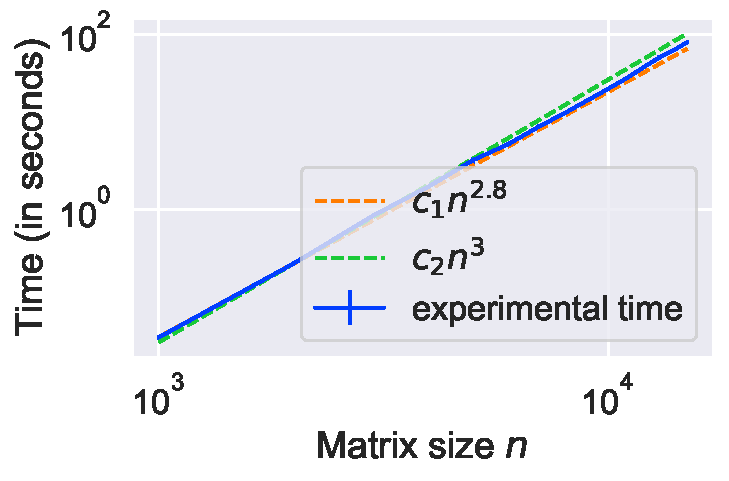
\includegraphics[width=\linewidth]{execution_time_solve}
        \end{minipage}
        %\includegraphics[width=0.4\linewidth]{execution_time_inversion}
        %&\includegraphics[width=0.4\linewidth]{execution_time_multiplication}\\
        &\begin{minipage}{0.45\linewidth}
            \begin{tabular}{|c|c|}
                \hline
                $n$ & Time (in second)\\\hline
                1000 & $ 0.03\pm0.02$ \\
                2000 & $ 0.24\pm0.01$ \\
                4000 & $ 1.83\pm0.05$ \\
                5000 & $ 3.6\pm0.3$ \\
                7000 & $ 8.7\pm0.5$ \\
                10000 & $23.7\pm0.6$ \\
                13000 & $54.0\pm2.5$ \\
                15000 & $80.8\pm1.8$ \\                
                \hline
            \end{tabular}
        \end{minipage}
    \end{tabular}
    \caption{Time taken of the default implementations \texttt{scipy.linalg.solve} of scipy to solve a linear system $\mA\mX=\mB$ where $\mA$ and $\mB$ are two square $n\times n$ matrices.}
    \label{fig:benchmark_inverse}
\end{figure}

%%%%%%%%%%%%%%%%%%%%%%%%%%%%%%%%%%%%%%%%%%%%%%%%%%%%%%%%%%%%%%%%%%%%%%%%%%%%%%%%%%%%%%%%%%%%%%%%%%%
%%%%%%%%%%%%%%%%%%%%%%%%%%%%%%%%%%%%%%%%%%%%%%%%%%%%%%%%%%%%%%%%%%%%%%%%%%%%%%%%%%%%%%%%%%%%%%%%%%%
\section{Detailed comparison with \texorpdfstring{\cite{akbarzadeh2020conditions} and \cite{nino2020fast}}{Akbarzadeh et al. 2020 and Nino Mora 2020.}}
\label{apx:comparison}

In this section, we compare our algorithm with two main related works for finite-state restless bandits problem.

\subsection{Comparison with \texorpdfstring{\cite{akbarzadeh2020conditions}}{Akbarzadeh2020 et al. 2022}}
The paper presents an  algorithm that computes Whittle indices  in $O(n^3)$ (no explicit constant before $n^3$ is given) for all indexable problems. Despite following a different approach, our algorithm for computing Whittle index can be viewed as a refinement of this work. Let us recall once again that our approach also allows one to check the indexability of general restless bandits.

In the following, we show how we can refine the work of \cite{akbarzadeh2020conditions} to obtain an algorithm that is exactly the same as ours.
%Let $\Phi^\pi$ be a square matrix and $D^{\pi}$ and $N^{\pi}$ be two vectors defined as in \cite{akbarzadeh2020conditions},
Let $D^{\pi}$ and $N^{\pi}$ be two vectors defined as in \cite{akbarzadeh2020conditions} (we use the same notation,  $D^{\pi}$ and $N^{\pi}$, as the cited paper),
\begin{align*}
    %\Phi^\pi = (I-\beta P^\pi)^{-1}, \quad
    D^{\pi} =(1-\beta)(\mI-\beta \mP^\pi)^{-1}\vr^{\pi}, \quad\text{and}\quad
    N^{\pi} =(1-\beta)(\mI-\beta \mP^\pi)^{-1}\vpi.
\end{align*}
Then, we have $D^{\pi} -\widx N^{\pi}=(1-\beta)\vu^{\pi}(\widx)$ where $\vu^{\pi}(\widx)$ is defined as in \eqref{eq:h is linear discounted}. In our proposition, at each iteration $k$, we compute $\mu_i^k$ by Line~\ref{algo2:muki}. Instead, it is defined in \cite{akbarzadeh2020conditions} by two steps:
\begin{enumerate}
\item for all state $j\in[n]$ such that $N_j^{\pi^k\setminus\{i\}}{\neq} N_j^{\pi^k}$, one needs to compute $\mu^k_{ij}{=}\displaystyle\frac{D_j^{\pi^k\setminus\{i\}} -D_j^{\pi^k}}{ N_j^{\pi^k\setminus\{i\}} -N_j^{\pi^k}}$ 
\item \label{it:mu^k_i*} compute $\mu^k_i=\displaystyle\argmin_{j\in[n]:N_j^{\pi^k\setminus\{i\}}\neq N_j^{\pi^k}} \mu^k_{ij}$.
\end{enumerate}
From \cite[Theorem 2]{akbarzadeh2020conditions}, in an indexable problem, for state $\sigma^k$, there exists a state $j\in[n]$ such that $N_j^{\pi^k\setminus\{\sigma^k\}}\neq N_j^{\pi^k}$. Now, suppose that for any active state $i\in\pi^k$, there exists $j\in[n]$ such that $N_j^{\pi^k\setminus\{i\}}\neq N_j^{\pi^k}$. Using the Sherman-Morrison formula, we have\footnote{the expression of $D^{\pi\setminus\{i\}}$ and $N^{\pi\setminus\{i\}}$ given by Equation~$(18)$ in \cite{akbarzadeh2020conditions} are erroneous.}
\begin{align*}
    &D^{\pi^k\setminus\{i\}} -D^{\pi^k} = -\frac{(1-\beta)\delta_i +\tilde{\mDelta}_iD^{\pi^k}}{1+\tilde{\mDelta}_i[(\mI-\beta \mP^{\pi^k})^{-1}]_{: i}}[(\mI-\beta \mP^{\pi^k})^{-1}]_{: i}, \\
    &\quad \text{and}\quad N^{\pi^k\setminus\{i\}} -N^{\pi^k} = -\frac{(1-\beta) +\tilde{\mDelta}_iN^{\pi^k}}{1+\tilde{\mDelta}_i[(\mI-\beta \mP^{\pi^k})^{-1}]_{: i}}[(\mI-\beta \mP^{\pi^k})^{-1}]_{: i}.
\end{align*}
Then, for any $j\in[n]$ such that $N_j^{\pi^k\setminus\{i\}}\neq N_j^{\pi^k}$, $\mu^k_{ij}=\displaystyle\frac{(1-\beta)\delta_i +\tilde{\mDelta}_iD^{\pi^k}}{(1-\beta) +\tilde{\mDelta}_iN^{\pi^k}}$ which does not depend on $j$.
Then, we simply have ${\mu^k_i=\displaystyle\frac{(1-\beta)\delta_i +\tilde{\mDelta}_iD^{\pi^k}}{(1-\beta) +\tilde{\mDelta}_iN^{\pi^k}}}$. %=\frac{\tilde{\Delta}_i((1-\beta)\vu^{\pi^k}(\mu^k_i)+\mu_i^kN^{\pi^k})}{\tilde{\Delta}_iN^{\pi^k}}$.
Also, we have 
\begin{align*}
    \tilde{\mDelta}_iN^{\pi^k}&=(1-\beta)\tilde{\mDelta}_i(\mI-\beta \mP^{\pi^k})^{-1}\vpi^k=-(1-\beta)y^k_i \quad\text{and}\\
    \tilde{\mDelta}_iD^{\pi^k}&={(1-\beta)\tilde{\mDelta}_i\vu^{\pi^k}(\mu^{k-1}_{\min}) +\mu^{k-1}_{\min}\tilde{\mDelta}_i N^{\pi^k}} =(1-\beta)z^{k-1}_i -(1-\beta)\mu^{k-1}_{\min}y^k_i.
\end{align*}
So, replacing these terms in $\mu^k_i$, we get the formula in Equation~\eqref{eq:mu^k_i_from_y} of our work.

Note that the algorithm of \cite{akbarzadeh2020conditions} was only developed for the discounted case.  Our approach for the time-average reward case is different because we use the active advantage function defined in \eqref{eq:advantage} instead of working with the expected discounted total reward $D^{\pi^k}$ and total number of activations $N^{\pi^k}$ under policy $\pi^k$. 
Note that the counterpart of $D^{\pi^k}$ in undiscounted MDP is the average reward $g^{\pi^k}$ and as we have seen in Appendix~\ref{apx:discussion_index}, utilizing average reward optimality is not rich enough for undiscounted MDPs with transient states.
In addition, our code is also optimized to avoid unnecessary computation and to reduce memory usage. Finally, the way we do the update of our matrix $\mX$ makes it possible to obtain a subcubic algorithm whereas their approach does not (see also below).

\subsection{Comparison with the algorithm of \texorpdfstring{\cite{nino2020fast}}{Nino Mora 2020}}
The algorithm \cite{nino2020fast} has the best complexity up to date for discounted restless bandit. There is a square matrix $\mA$ that plays a similar role as the square matrix $\mX$ in our proposed algorithm. The most costly operations in the algorithm of \cite{nino2020fast} is to update their matrix $\mA$ at each iteration and it is done by Equation~\eqref{eq:update_X_naif} that we recall here (using the same notation $\mA$ as the cited paper):
\begin{align}
    \label{eq:15}
    \text{for } i,j\in\pi^k,\ \mA^{k+1}_{ij}= \mA^{k}_{ij} -\frac{\mA^{k}_{i\sigma^k}}{\mA^{k}_{\sigma^k\sigma^k}}\mA^{k}_{\sigma^kj}.
\end{align}
This incurs a total complexity of $(2/3)n^3+O(n^2)$ arithmetic operations.
As mentioned in Section~\ref{ssec:two_third_algo}, if we updated $\mX^{k+1}$ as given by \eqref{eq:update_X_naif}, our algorithm would also have a $(2/3)n^3+O(n^2)$ complexity but this version of update cannot be optimized by using  fast matrix multiplication.

\subsection{Their approach cannot be directly transformed into a subcubic algorithm}
\label{apx:eq_15}

In addition to all the previously cited differences, one of the major contribution of our algorithm with respect to \cite{akbarzadeh2020conditions,nino2020fast} is that the most advanced version of our algorithm runs in a subcubic time. The approach\footnote{Equation~(18) of \cite{akbarzadeh2020conditions}, which is central to their algorithm is the same as the above equation \eqref{eq:15}.} used  in \cite{akbarzadeh2020conditions,nino2020fast} is to update the full matrix $\mX^{k+1}$ at iteration $k$, by using \eqref{eq:15}.  This idea is represented in Figure~\ref{fig:apx_fast_mm}(a): for a given $\ell$, their algorithm compute $\mX^\ell_{:\sigma^k}$ for all $k$ (i.e., the full vertical lines represented by arrows).  Our first Subroutine~\ref{algo:update_X} uses an horizontal approach based on \eqref{eq:X^ell+1-i}, which we recall here:
\begin{align*}
    X^{\ell+1}_{i\sigma^k} &= X^{\ell}_{i\sigma^k} - \frac{X^{\ell}_{i\sigma^\ell}}{1+X^{\ell}_{{\sigma^\ell\sigma^\ell}}} X^{\ell}_{{\sigma^\ell} \sigma^k}.
\end{align*}
At iteration $k+1$, we use $\mX^{1}_{: \sigma^k}$ to compute all values of $\mX^\ell_{:\sigma^k}$ up to $\ell=k+1$.  This is represented in Figure~\ref{fig:apx_fast_mm}(b).  Our approach can be used to obtain the subcubic algorithm illustrated in Figure~\ref{fig:apx_fast_mm}(c) by using subcubic algorithms for multiplication.


\begin{figure}[ht]
    \centering
    \begin{tabular}{ccc}
        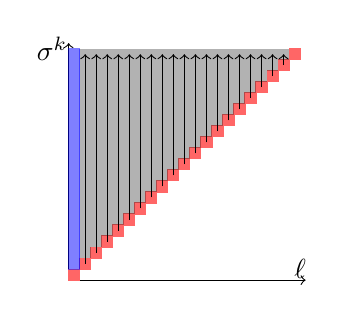
\begin{tikzpicture}[scale=0.14, shorten >=2pt]
            \draw (0,0) edge[->] (22,0);
            \draw (0,0) edge[->] (0,22);
            \node at (21,1) {$\ell$};
            \node at (-1.5,21) {$\sigma^k$};
            \foreach \i in {0,...,20} \draw[fill,red!60] (\i,\i) rectangle (\i+1,\i+1);
            \foreach \i in {0}{
               \draw[fill,blue,opacity=0.5] (\i,\i+1) rectangle (\i+1,21);
               \foreach \j in {1,...,19}{
                   \fill[black,opacity=0.3] (\i+\j,\i+\j+1) rectangle (\i+\j+1,\i+21);
               }
            }
            \foreach \i in {1,...,19}{
                \draw (\i+0.5,\i+0.5) edge[->] (\i+0.5,21);
            }
        \end{tikzpicture}
        &
        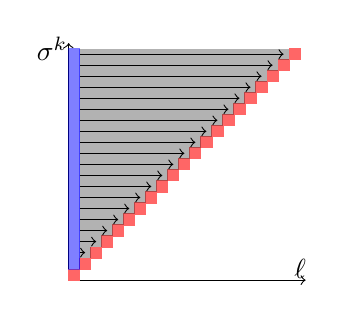
\begin{tikzpicture}[scale=0.14, shorten >=2pt]
            \draw (0,0) edge[->] (22,0);
            \draw (0,0) edge[->] (0,22);
            \node at (21,1) {$\ell$};
            \node at (-1.5,21) {$\sigma^k$};
            \foreach \i in {0,...,20} \draw[fill,red!60] (\i,\i) rectangle (\i+1,\i+1);
            \foreach \i in {0}{
               \draw[fill,blue,opacity=0.5] (\i,\i+1) rectangle (\i+1,21);
               \foreach \j in {1,...,19}{
                   \fill[black,opacity=0.3] (\i+\j,\i+\j+1) rectangle (\i+\j+1,\i+21);
               }
            }
            \foreach \i in {2,...,20}{
                \draw (1,\i+0.5) edge[->] (\i,\i+0.5);
            }
        \end{tikzpicture}
        &
        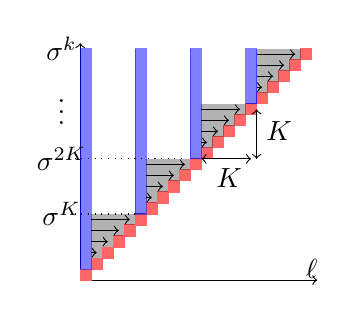
\begin{tikzpicture}[scale=0.14, shorten >=2pt]
            \draw (0,0) edge[->] (22,0);
            \draw (0,0) edge[->] (0,22);
            \node at (21,1) {$\ell$};
            \node at (-1.7,21) {$\sigma^k$};
            \foreach \i in {0,...,20} \draw[fill,red!60] (\i,\i) rectangle (\i+1,\i+1);
            \foreach \i in {0,5,10,15}{
               \draw[fill,blue,opacity=0.5] (\i,\i+1) rectangle (\i+1,21);
               \foreach \j in {1,...,5}{
                   \fill[black,opacity=0.3] (\i+\j,\i+\j+1) rectangle (\i+\j+1,\i+6);
                }
                \foreach \j in {2,...,5}{
                    \draw (\i+1,\i+\j+0.5) edge[->] (\i+\j,\i+\j+0.5);
                }
            }
            \draw (11,11) edge[<->] node[below] {$K$} (16,11);
            \draw (16,11) edge[<->] node[right] {$K$} (16,16);
            \node at (-1.7,6) {$\sigma^K$}; \draw[dotted] (-.5,6) -- (5.5,6);
            \node at (-1.7,11) {$\sigma^{2K}$}; \draw[dotted] (-.5,11) -- (10,11);
            \node at (-1.7,16) {$\vdots$};
        \end{tikzpicture} \\
        (a) \cite{akbarzadeh2020conditions,nino2020fast} use \eqref{eq:15}.
        &(b) Subroutine~\ref{algo:update_X}.
        &(c) Subroutine~\ref{algo:FMM}.
    \end{tabular}
    \caption{Comparison of the computation load of \eqref{eq:15} used in \cite{akbarzadeh2020conditions,nino2020fast} with the one of Subroutine~\ref{algo:update_X} and Subroutine~\ref{algo:FMM}. }
    \label{fig:apx_fast_mm}
\end{figure}

This  leads to the next fundamental  question: {why should the computation of Whittle index be harder than matrix inversion (or multiplication)?} To us, the main difference is that when computing Whittle indices, the permutation $\sigma$ is not known a priori but discovered as the algorithm progresses: $\sigma^k$ is only known at iteration $k$. Hence, while all terms of the matrices $X^k_{ij}$ are not needed, it is difficult to know a priori which ones are needed and which ones are not. Hence, a simple divide and conquer algorithm cannot be used. This is why when recomputing $\mX^{k+1}$ in Subroutine~\ref{algo:FMM}, we recompute the whole matrix (the vertical blue line) and not just the part that  will be used to compute the gray zone: we do not know \emph{a priori} what part of $X^{k+1}_{ij}$ will be useful or not.

\endgroup

\chapter{Carbon footprint}
\label{chapter:blabla2}

\lipsum[11-12]

